\documentclass{beamer}
\usetheme{Zurich}
\usepackage{amsmath, amsfonts, graphicx, multirow}
\title{Classification and Regression Trees}
\author{Charlotte Wickham}
\date{\today}

\begin{document}

\frame{\titlepage}

\section[Outline]{ 	}
\frame{\tableofcontents}


\begin{frame}
	\frametitle{Trees}
	\begin{itemize}
		\item Restrict to binary splits
		\item Computationally infeasible to build every possible tree
		\item Want a algorithm that builds a ``good'' tree.
	\end{itemize}
\end{frame}


\begin{frame}
	\frametitle{Trees}
	Two components:
	\begin{itemize}
		
		\item Growing trees
		\item Pruning trees
		
	\end{itemize}
\end{frame}

\begin{frame}
\frametitle{Basic Idea}
Growing trees:
\begin{itemize}
	\item Choose the ``best'' possible binary split of the data
	\item Take each side of the split and find the next ``best'' split for each side.
	\item Continue until either each terminal node is ``pure'' or of some minimum size.
\end{itemize}
Will result in an over-fitted tree. Then need to prune tree:
\begin{itemize}
	\item Using large tree prune back to find ``best'' tree of various sizes
	\item Use cross-validation to choose ``best'' size.
\end{itemize}
\end{frame}
\section{Growing trees}
\begin{frame}
	\frametitle{Growing trees}
	Need four things:
	\begin{itemize}
		\item A set of possible splits
		\item A measure of how good a split is
		\item A stop-splitting rule
		\item A rule for assigning a terminal node to a class. 
	\end{itemize}
\end{frame}


\begin{frame}
	\frametitle{Growing trees - Possible splits}
	Only split on one variable:
	\begin{itemize}
		\item Binary variables 
		\begin{itemize}
			\item one possible binary split
		\end{itemize}
		\item Categorical variables
		\begin{itemize}
			\item Splits of the form $x \in S$ where $S$ could be any possible subset of the categorical levels.
			\item  $2^{L-1} - 1$ possible splits.
		\end{itemize}
		\item Continuous or ordinal variables 
		\begin{itemize}
			\item Splits of the form $x \le x_c$.
			\item  At most N possibilities  - where $x_c$ is halfway between to consecutive distinct values.
		\end{itemize}   
	\end{itemize}
	Need a measure to choose which spilt is best.
\end{frame}

\begin{frame}
	\frametitle{Growing trees - Best split}	
	Introduce an impurity function $f$.
	
	Let the impurity of a node $t$ be, 
	\[
	I(t) = \sum_{i=1}^C f(p_{it}),
	\]
	where $p_{it}$ is the proportion of those in $t$ that belong to class $i$ in future samples (in practice use the proportions in the learning set possibly times a prior).
	
	\begin{itemize}
		\item Want $I(t)$ to be maximal when node contains equal amounts of each class.
		\item Want $I(t)$ to be minimal (i.e. 0) when node contains only one class.
	\end{itemize}
\end{frame}

\begin{frame}	
\frametitle{Growing trees - Best split}	
Given a split, $s$, that sends a proportion $p_R$ of the data to $t_R$ and $p_L$	to $t_L$ the decrease in impurity from the split is, 
	\[
	\Delta I(s,t) = I(t) - p_RI(t_R) - p_LI(t_L)
	\]
Want to choose a split that maximises this decrease.

Some examples of f:
\begin{itemize}
	\item Gini index $f(p) = p(1-p)$
	\item Information index $f(p) = -p\log{p}$
\end{itemize}
\end{frame}


\begin{frame}
	\frametitle{Growing trees - Stopping rule \& assigning classes}	
	Stopping rule
	\begin{itemize}
		\item Want a large tree - since we are going to prune later
		\item Keep growing until either terminal nodes are very small or are pure.
	\end{itemize}
	Assigning classes
	\begin{itemize}
		\item Assign to the class with the largest $p_{it}$ 
	\end{itemize}
	
\end{frame}

\section{Pruning trees}
\begin{frame}
	\frametitle{Pruning}
\begin{itemize}

	\item 	We now have a large tree which will have likely over-fitted the data.  We want to prune back to a smaller tree.
	\item 	Basically, define a cost-complexity measure that is the misclassification cost of a tree penalized by its complexity.
	\begin{itemize}
	\item 	cost-complexity of $T$ = misclassification rate of $T$ $+ \alpha |T|$.
	\item 	$|T|$ is the number of terminal nodes and measures the complexity of tree $T$.
\end{itemize}
	\item  Find $T$ that minimises the cost-complexity for various $\alpha$.	
\end{itemize}
Turns out this defines a sequence of nested subtrees of our original large tree.

\end{frame}

\begin{frame}
	\frametitle{Choosing the level of pruning}
	\begin{itemize}
		\item How do we choose the best sized tree from the sequence generated?
		\item Want to minimise the misclasification rate
		\item Misclassification rate on the training data will always decrease with increasing tree size
		\item Need an estimate if the misclassification rate for new data
		\item Cross validation!
	\end{itemize}
\end{frame}


\section{Supernova}
\begin{frame}
	\frametitle{Supernova Data}
	\begin{itemize}
		\item 5000 Supernova and 5000 other objects
		\item Split into two sets 9000 in training 1000 in test
		\item Build tree and prune based on training set using cross validation
		\item Test prediction on test set and compare to support vector machines.
	\end{itemize}
\end{frame}


\begin{frame}
\frametitle{Growing full length tree}
\setkeys{Gin}{width=\textwidth}
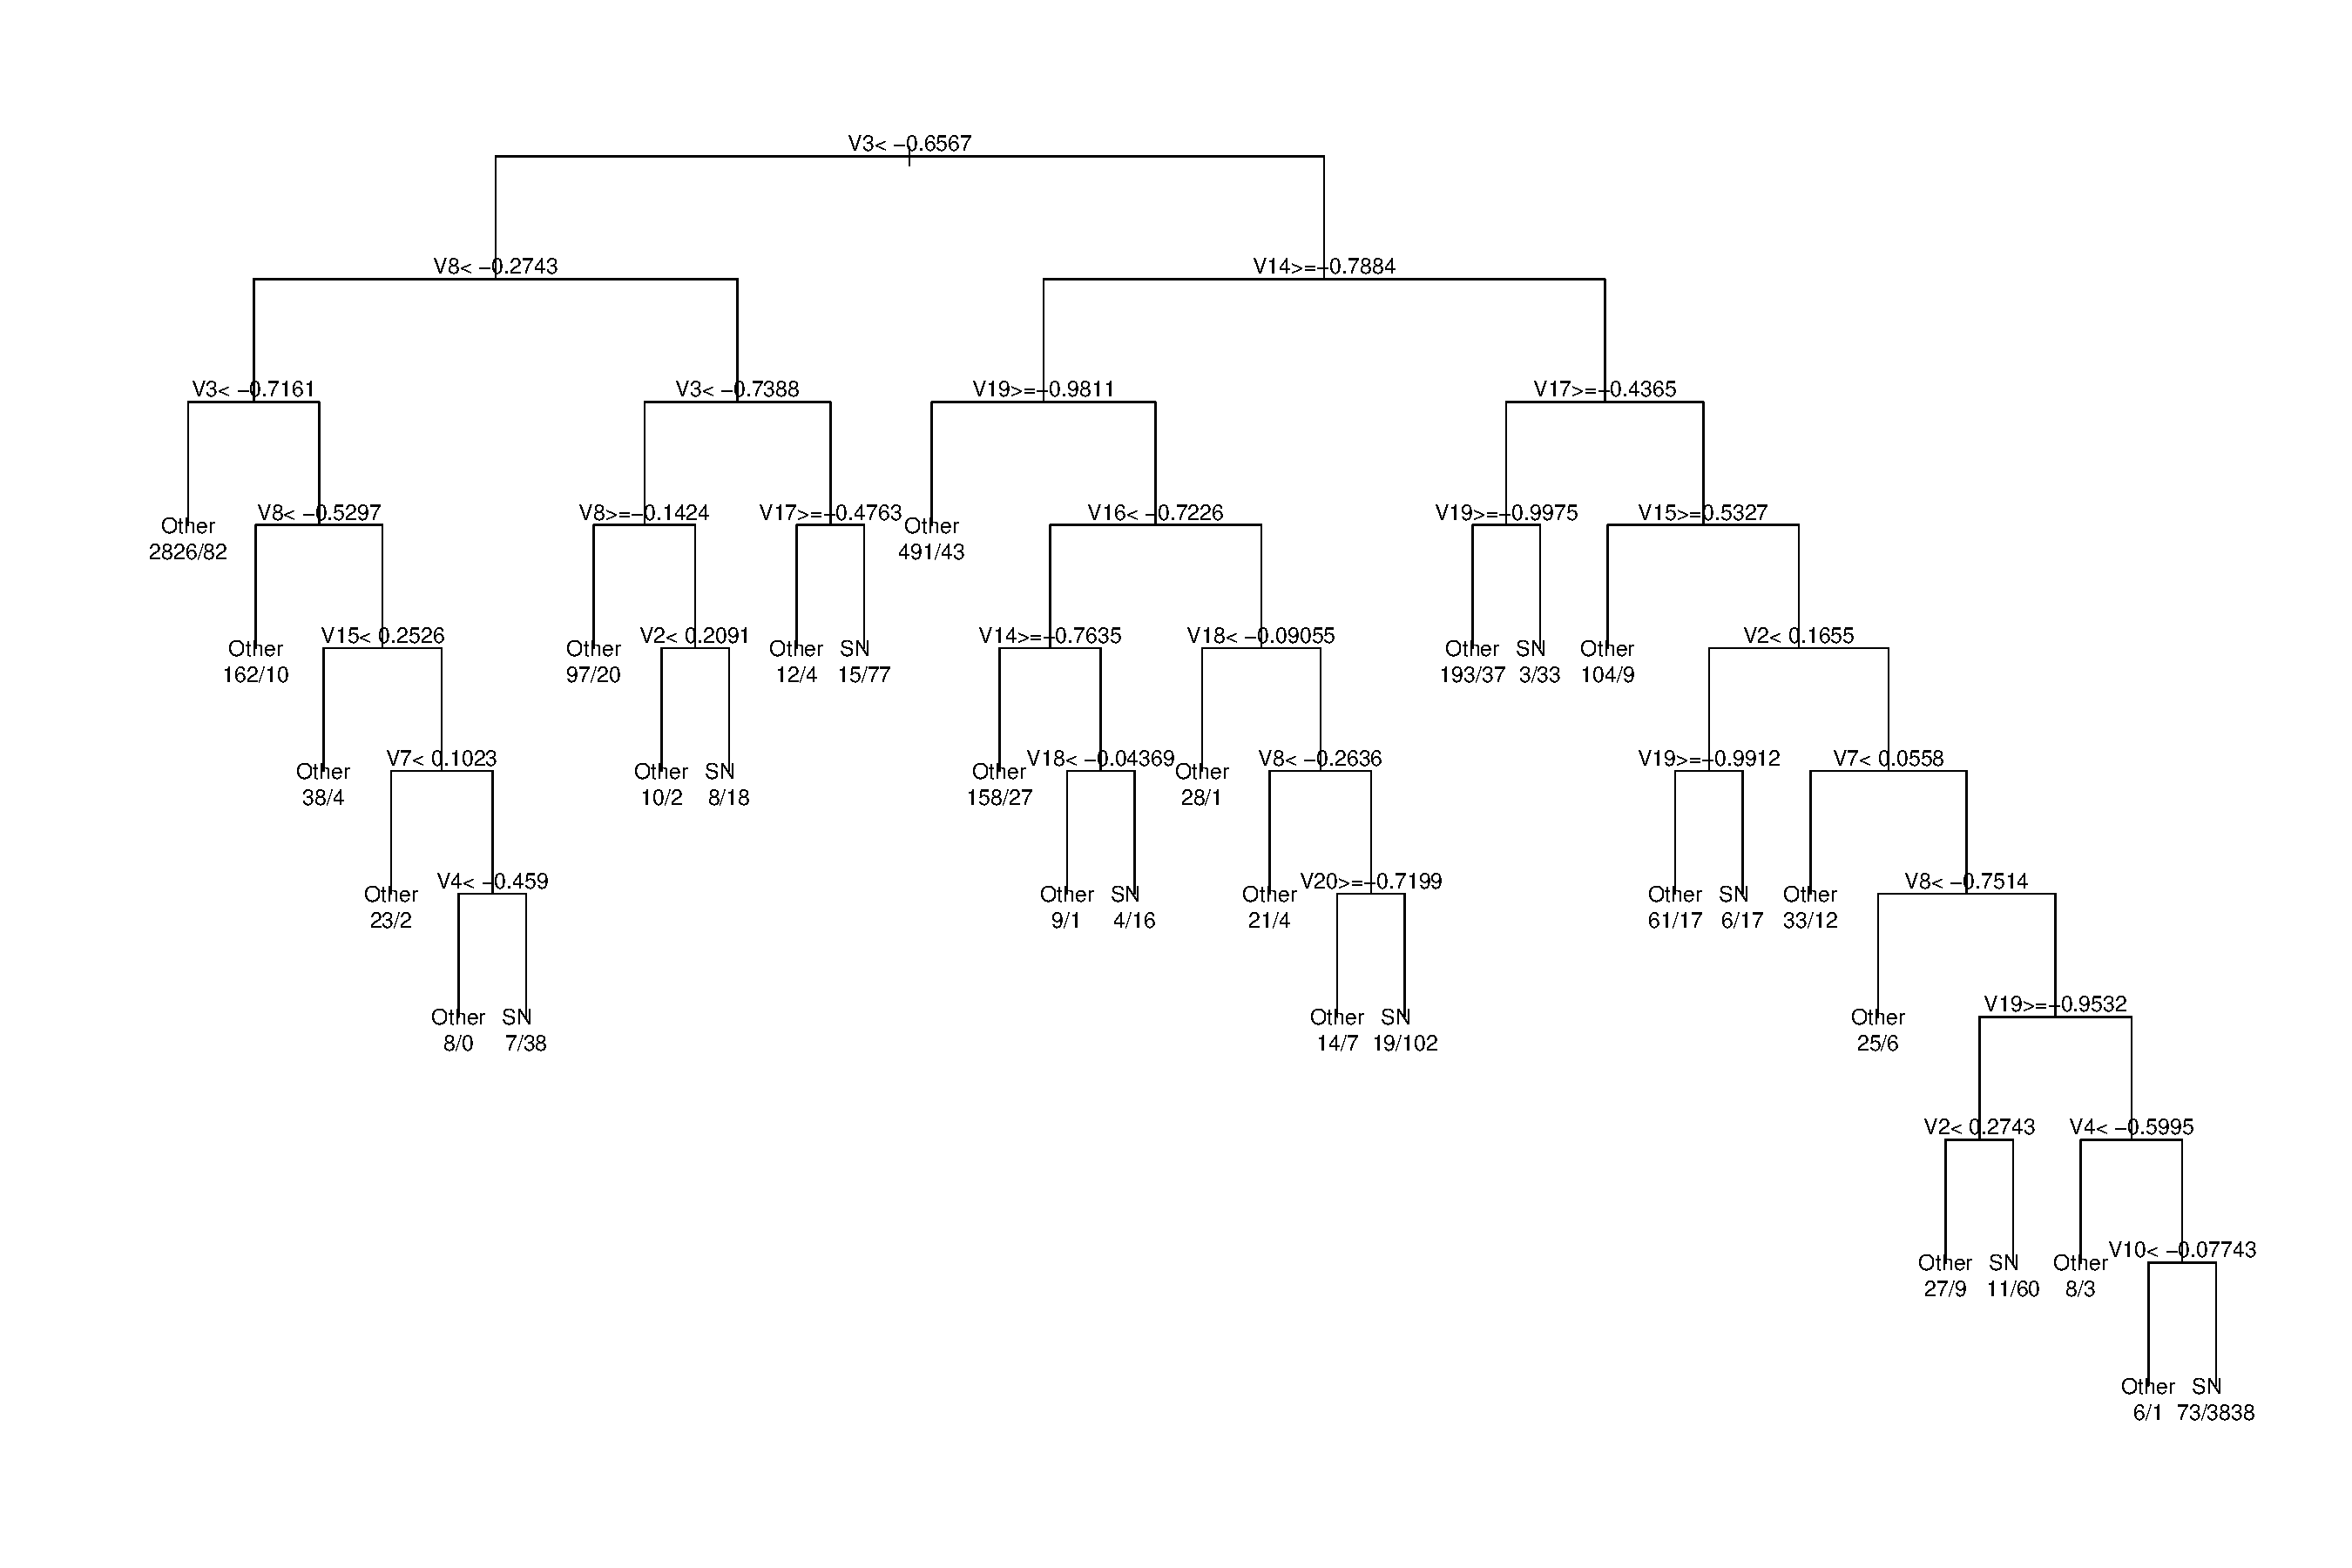
\includegraphics{full.pdf}
\end{frame}



\begin{frame}
\frametitle{Pruning}
\begin{columns}[c] % the "c" option specifies center vertical alignment 
	\column{.6\textwidth} % column designated by a command
\setkeys{Gin}{width=\textwidth}
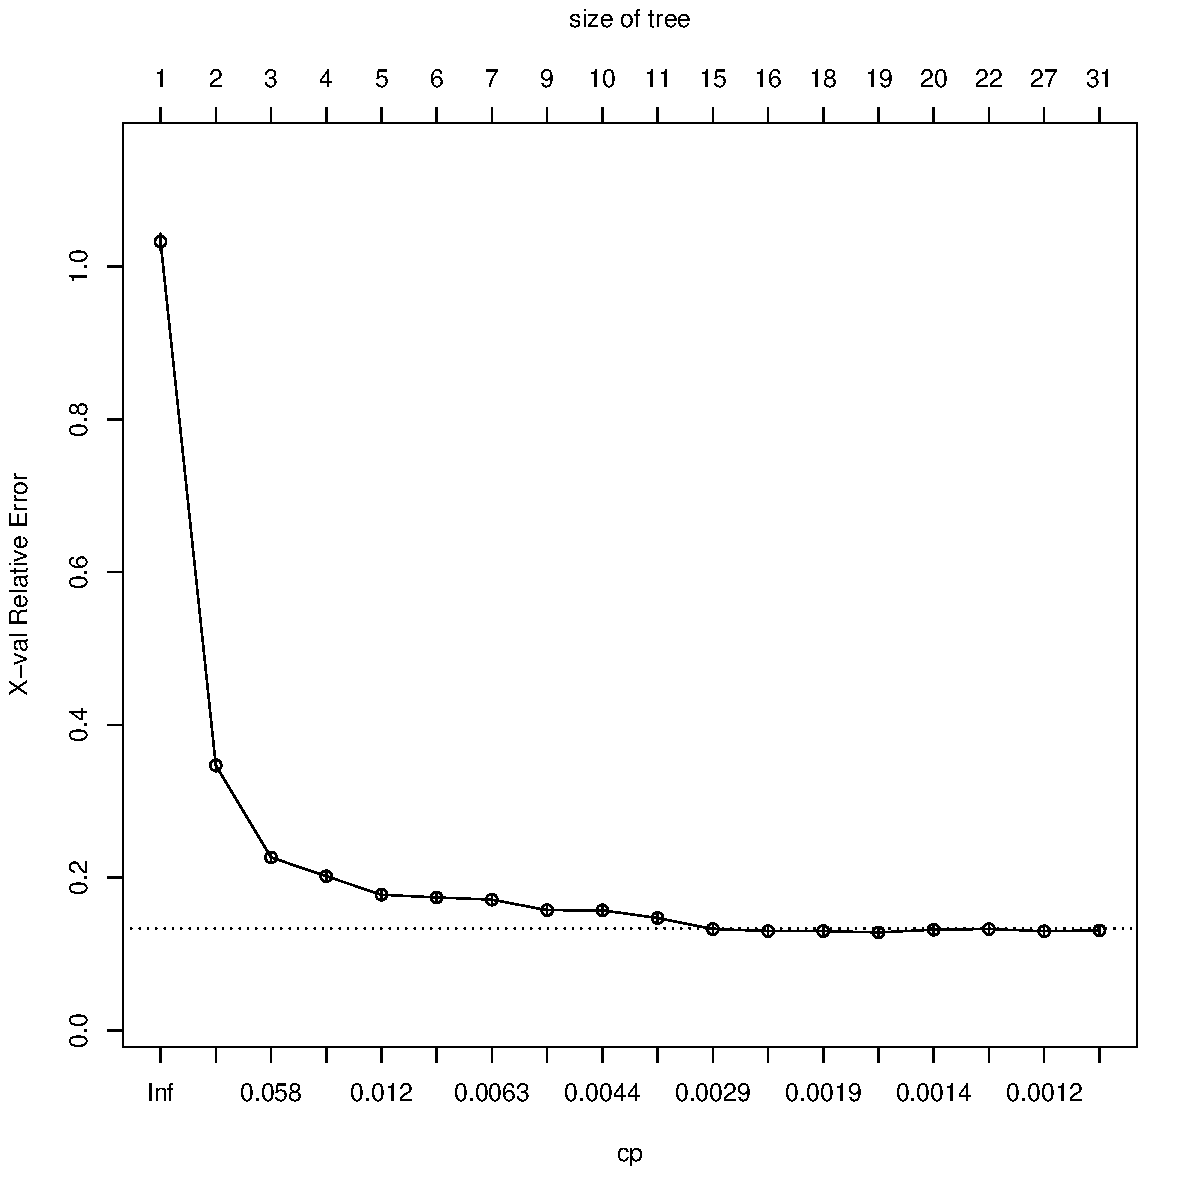
\includegraphics{cp.pdf}
	\column{.4\textwidth}
	\begin{itemize}
		\item Look for smallest tree within 1sd of tree with minimum  error. 
		\item About 14 splits.
	\end{itemize}
	\end{columns}
\end{frame}

\begin{frame}
\frametitle{Pruned tree}
\setkeys{Gin}{width=\textwidth}
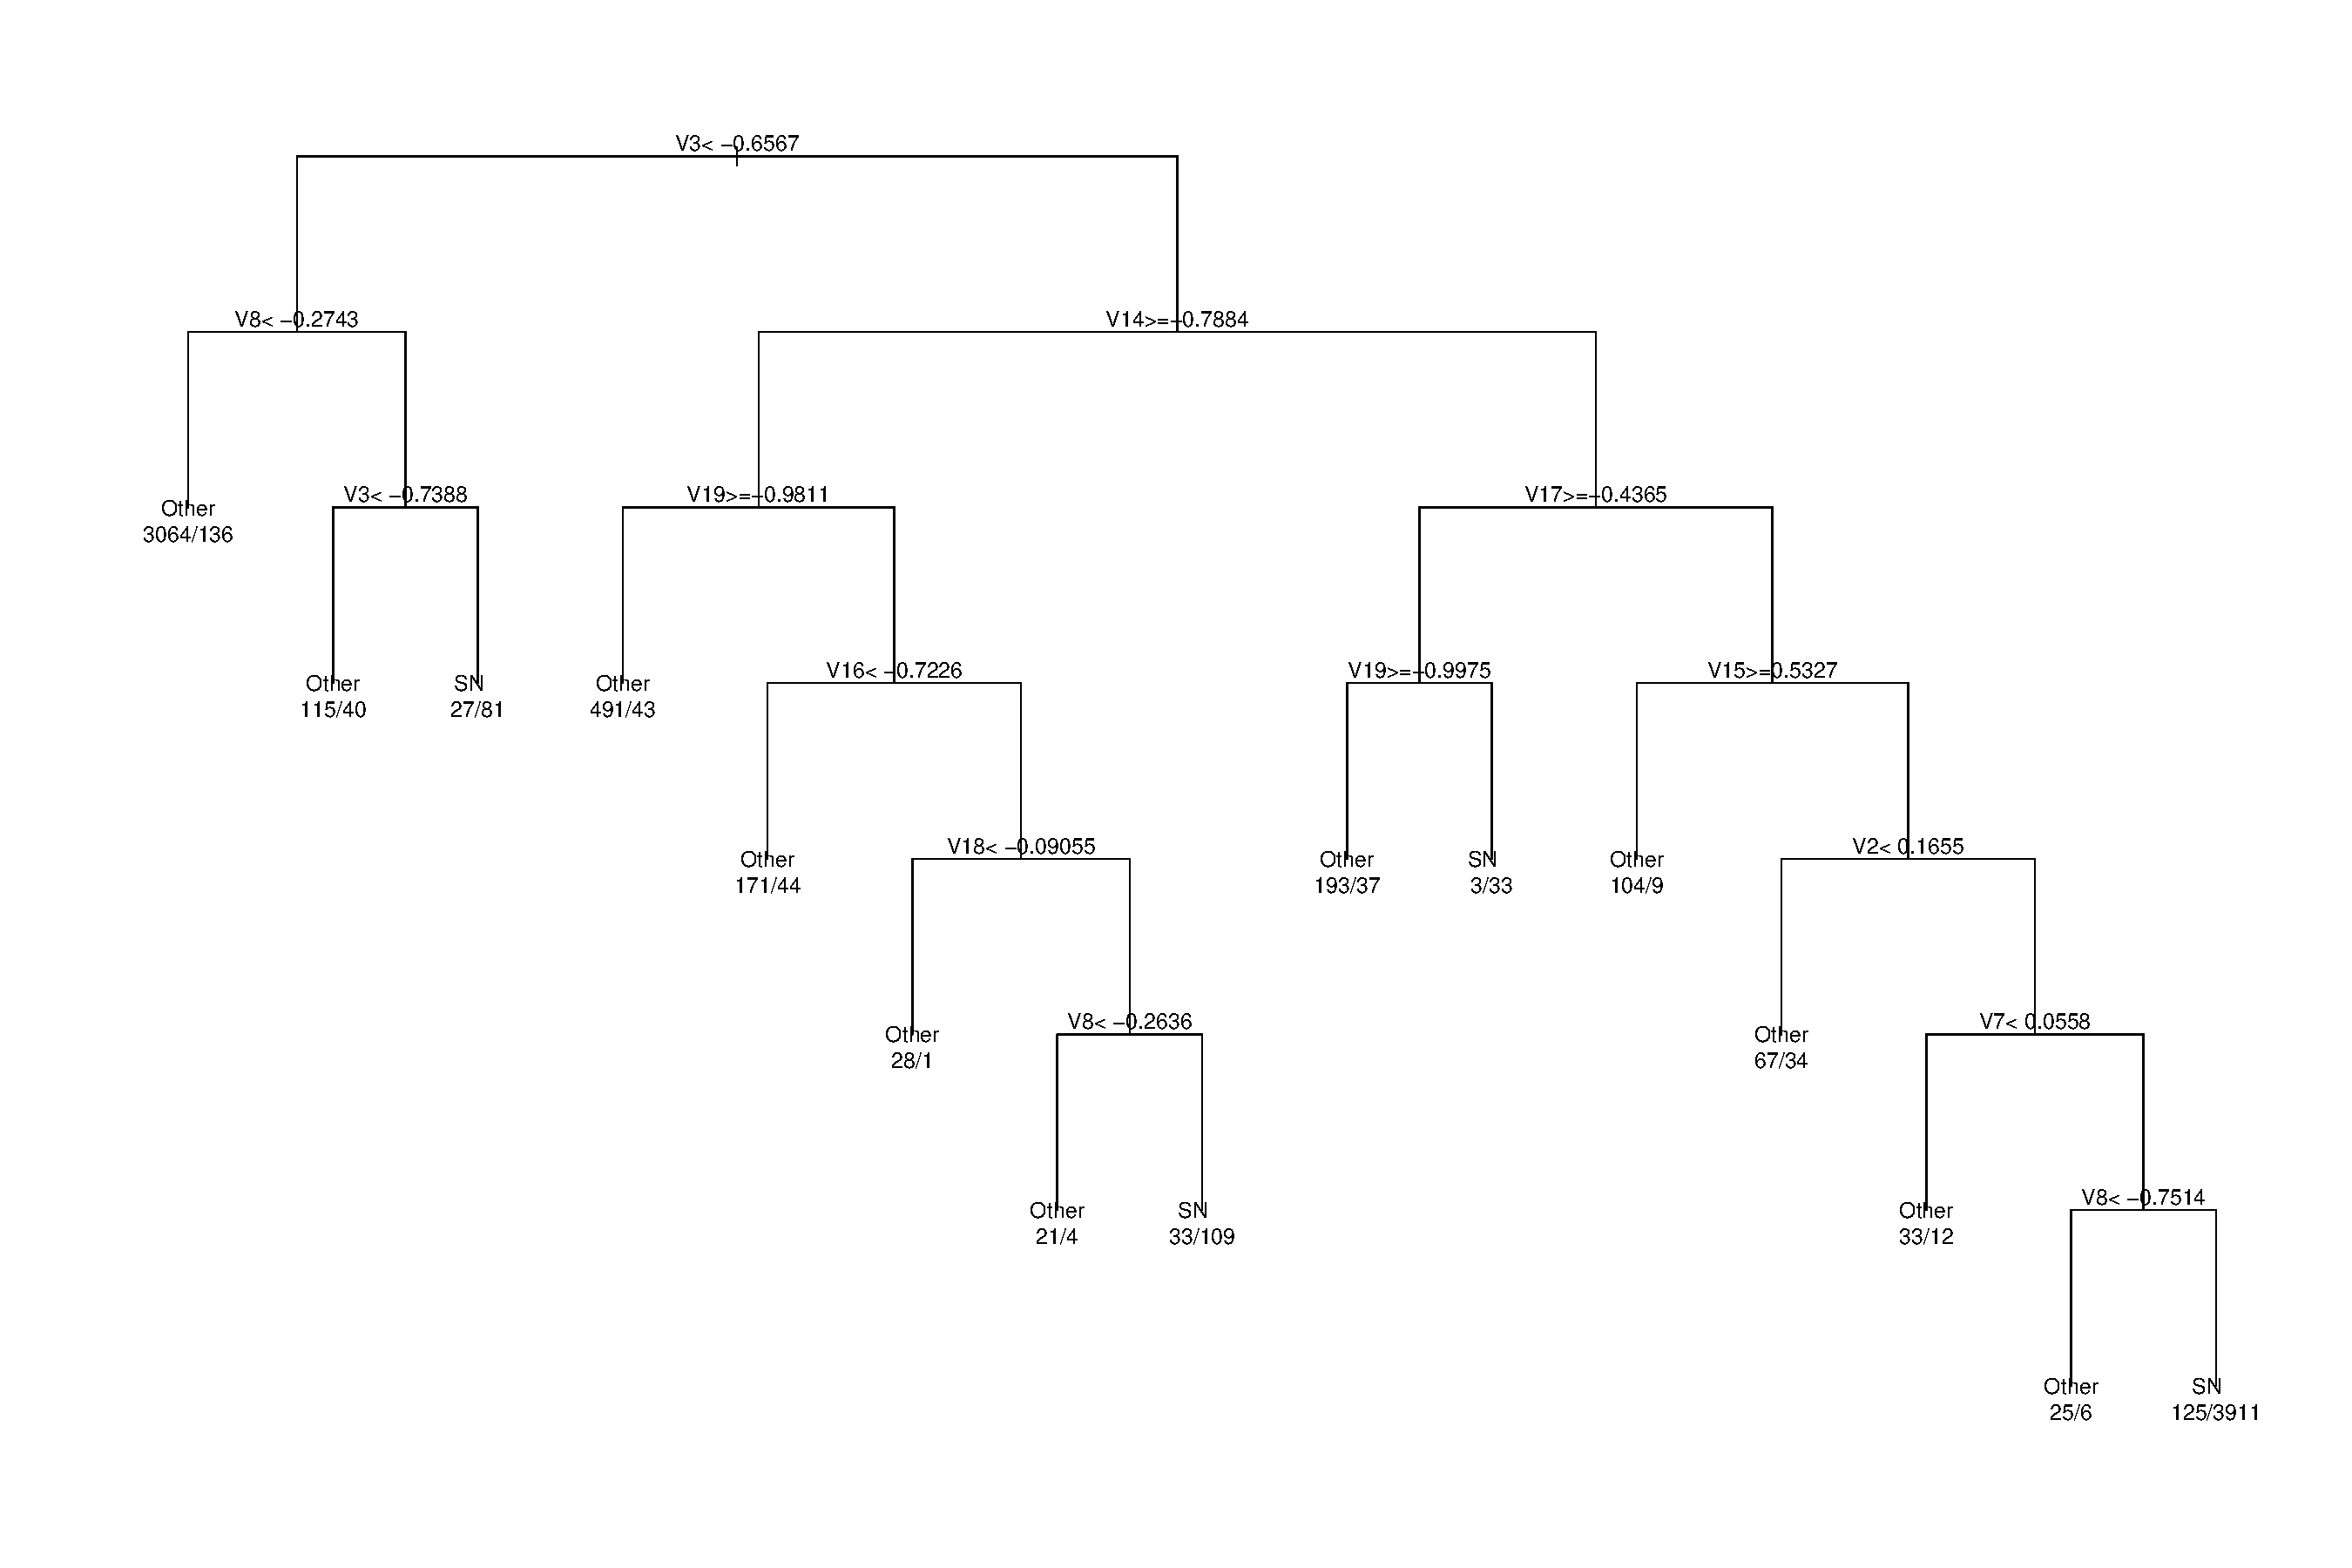
\includegraphics{tree.pdf}
\end{frame}

\begin{frame}
\frametitle{Left branch}
\setkeys{Gin}{width=0.8\textwidth}
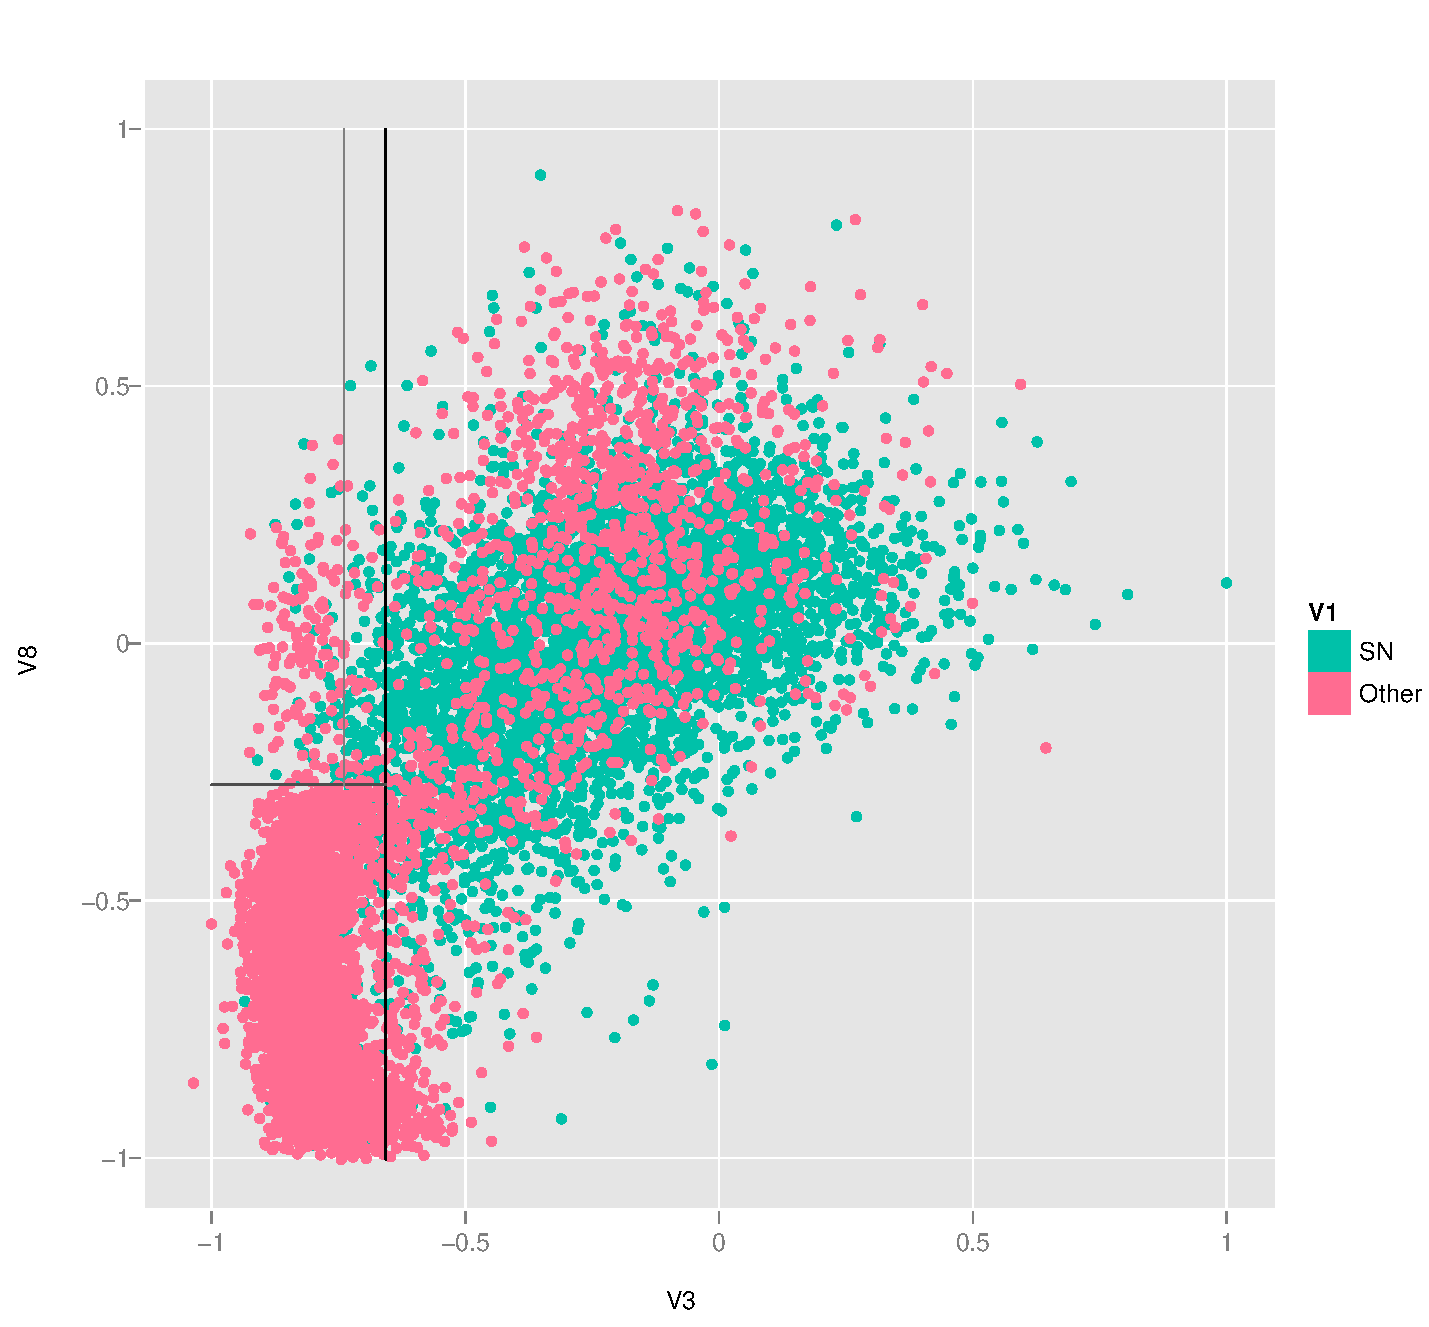
\includegraphics{leftside.pdf}
\end{frame}

\begin{frame}
	\frametitle{Performance on test set}
	\begin{itemize}
		\item{Classification Tree
		\begin{table}
		\begin{tabular}{cr|rr}
		& & \multicolumn{2}{c}{Prediction}\\
		& & Other & Supernova\\
		\hline
		\multirow{2}{*}{\rotatebox{90}{Actual}} & Other &  461 &  39\\
		& Supernova & 45 &  455\\
		\end{tabular}
		\end{table}
		Error = 8.4\%}
		
		\item{Best Support Vector Machine
		\begin{table}
		\begin{tabular}{cr|rr}
		& & \multicolumn{2}{c}{Prediction}\\
		& & Other & Supernova\\
		\hline
		\multirow{2}{*}{\rotatebox{90}{Actual}} & Other &  484 &  16\\
		& Supernova & 32 &  468\\
		\end{tabular}
		\end{table}
		Error = 4.8\%
		}
		
	\end{itemize}
\end{frame}

\begin{frame}
	\frametitle{Other things to look into}
	\begin{itemize}
		\item Try different impurity measures
		\item Using linear combination of variables as splits
		\item Priors?
	\end{itemize}
\end{frame}


\nocite{546466}
\nocite{rpart}
\nocite{cart84}

\frame{
\begin{tiny}
\bibliographystyle{plainnat}
\bibliography{refs}
\end{tiny}
}




\end{document}

